\documentclass[a4paper]{article}
\usepackage{preamble}

% Setup title
\title{MATHEMATICS 2 - TERM 2}
\author{Marc Sanchis}
\date{April 2024 - June 2024}

\begin{document}

% Title
\newgeometry{top=2cm, bottom=5.5cm}
\maketitle

% Table of Contents
\renewcommand{\contentsname}{}
\tableofcontents

% Body
\newpage
\restoregeometry
\pagestyle{fancy}

\section{Introduction to Differential Equations}

A differential equation (DE) is an equation containing one or more dependent variable derivatives, like \textit{Newton's Law}
$$
F=m \frac{d^{2}x(t)}{dt^{2}}=mx''=m\ddot{x}
$$

DEs with one independent variable are called \textbf{Ordinary Differential Equations} (ODE); an example can be the \textit{Radioactive Disintegration} $m'=km$, where $k$ is an independent variable.

DEs with multiple independent variables and partial derivatives are called \textbf{Partial Differential Equations}; an example can be the \textit{Wave Equation}
$$
\nabla u\equiv\nabla^{2}u=\frac{\partial^{2}u(\mathbf{x}, t)}{\partial x^{2}}+\frac{\partial^{2}u(\mathbf{x},t)}{\partial y^{2}}+\frac{\partial^{2}u(\mathbf{x},t)}{\partial z^{2}}=\frac{1}{c^{2}}\frac{\partial^{2}u(\mathbf{x},t)}{\partial t^{2}}
$$

\note{The largest order of derivative defines the order of the DE. An ODE is lineal for $F(t,y,y',\dots,y(n))=0$}

An ODE can be solved with a general ($=\dots+C$) or particular ($=\dots+k,\,k=\mathbb{R}$). The result can be given by an Initial Value Problem (IVP): a function $f(t)$ verifying the ODE and the Initial Condition (IC).

\note{Frontier problems are an IVP but verifying an IC relative to the contour, a Contour Condition (CC)}

\section{First Order Differential Equations}

\subsection{Separable DE}
A first-order ODE $F(t,y,y')$ is \textit{separable} if it can be written as
$$
A(t)dt=B(y)dy,\hspace{4ex}y'=\frac{A(t)}{B(y)},\hspace{4ex}y'=C(t)D(y)
$$

\textit{\textbf{Prob.:}} A bowl filled with water spins at a $w$ velocity. If we put a mass $m$ on the surface of the water and denote tension force by $T$, centrifugal force by $F_{c}$ and weight by $P$. Formulate Newton's Equation.

\begin{align}
F&=ma, & v&=cte\implies a=0 \\
F&=0, & \sum^{}_{}F&=P+F_{c}+T \\
0&= P+F_{c}+T
\end{align}
$$
P=-mg\mathbf{j},\, F_{c}=mR\omega 2i,\, T=-T\sin \alpha \mathbf{i} + T\cos \alpha \mathbf{j}
$$
Where $T=\mid\mid \mathbf{T}\mid\mid$ and $\alpha$ is the angle between the tangent and the horizontal axis

\begin{minipage}{0.4\textwidth}
equalling these terms
\begin{align}
\begin{cases}
T\sin \alpha=mR\omega^{2}, \\
T\cos \alpha=mg
\end{cases} \\
R\omega^{2}g=\tan \alpha
\end{align}
$$
\boxed{\frac{\omega^{2}}{g}x=\frac{dy}{dx}}
$$
\end{minipage} \hfill \begin{minipage}{0.4\linewidth}
\begin{figure}[H]
    \centering
    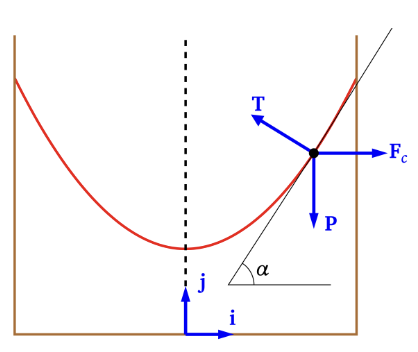
\includegraphics[width=\textwidth]{IMG/ex_water.png}
    \caption{Water bowl example}
    \label{fig:ex_water}
\end{figure}
\end{minipage}



\subsection{Homogeneous ODE}

\note{A function $f(x,y)$ is said to be of order $n$ if $f(\lambda x,\lambda y)=\lambda^nf(x,y)$}

A first-order ODE $M(x,y)dx+N(x,y)dy=0$ is homogeneous if and only if $M$ and $N$ are of the same order.

\note{Given a homogeneous ODE $dy / dt=f(t,y)$, it can be solved by making the change $u=y / t$ converting the equation into a separable variables equation}

\textit{\textbf{Ex.:}} $t^{3}y'=t^{2}y-2y^{3}$
\begin{align} 
y'=\frac{t^{2}y-2y^{3}}{t^{3}}&=\frac{y}{t}-2\left( \frac{y}{t} \right)^{3} \\
u&=y / t \\
f(y / t)&=f(u)=u-2u^{3} \\
y'=\frac{dy}{dt}&=\frac{d(ut)}{dt}=\frac{du}{dt}t+u \\
\frac{du}{dt}t+u&=u-2u^{3} \\
\frac{du}{2u^{3}}&=-\frac{dt}{t}
\end{align}

\textit{\textbf{Prob.:}} Find the form of a curved mirror that divides a beam of light parallel to the $X$ axis.

The beams will be reflected towards a point we will be calling $F$ (property of a parabolic antenna).

\begin{figure}[H]
    \centering
    \begin{subfigure}{0.3\textwidth}
        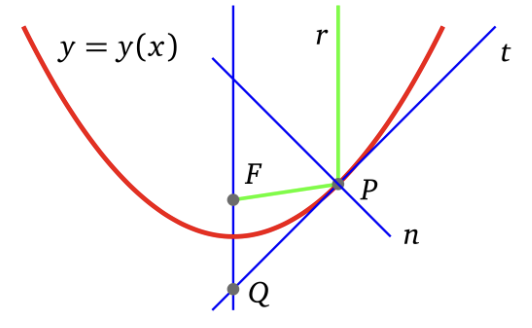
\includegraphics[width=\textwidth]{IMG/prob_mirror1.png}
    \end{subfigure}\hspace{5ex}
    \begin{subfigure}{0.3\textwidth}
        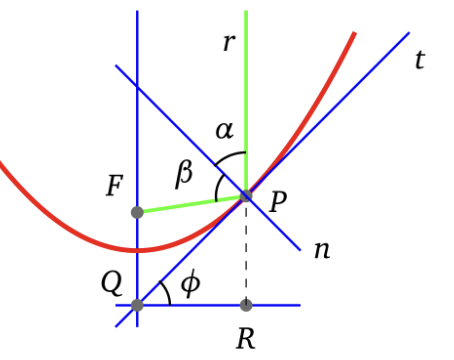
\includegraphics[width=\textwidth]{IMG/prob_mirror2.png}
    \end{subfigure}
    \caption{Parabolic mirror problem}
    \label{fig:prob_mirror}
\end{figure}

Let the axis through $\overline{FQ}$ be $y$, $P(x,y)$ is the intersection of the beam and the mirror, $t$ being its tangent and $n=\mid\mid t\times y(x)\mid\mid$ the normal. The angles denoted by $\alpha,\beta,\phi$. For $r \perp x \implies \phi=\alpha$, and following \textit{Snell's Law} $\alpha=\beta$, and by geometry $\alpha=\phi$, so $\alpha=\beta=\phi$. Knowing this, we can affirm that the triangle formed by $PQF$ is isosceles, implying $PF=FQ$.

$\phi=dy / dx=\frac{PR}{QR}$ and if we place $F$ on $(0,0)$, then $PR=y+FQ=y+\sqrt{ x^{2}+y^{2} }$ and $QR=x$, so
$$
\frac{dy}{dx}=\frac{y+\sqrt{ x^{2}+y^{2} }}{x}\hspace{4ex}\leftarrow\text{homogeneous}
$$
and we can make $u=y / x$
\begin{align}
\frac{d(ux)}{dx}&=\frac{ux+\sqrt{ x^{2}+(ux)^{2} }}{x}\implies \\
\implies&u+x \frac{du}{dx}=u+\sqrt{ 1+u^{2} }\implies \\
\implies&x \frac{du}{dx}=\sqrt{ 1+u^{2} } \implies
\end{align}
$$
\boxed{\frac{du}{\sqrt{ 1+u^{2} }}=\frac{dx}{x} \implies F(y / x)=\log x+C}
$$

\textit{\textbf{Ex.:}} Solve for $y'=(2y-t+1) / (t+y+3)$
\begin{align}
f(\lambda y,\lambda t)&=\frac{2\lambda y-\lambda t+1}{\lambda y+\lambda t+3}, & &\leftarrow\text{not homogeneous}
\end{align}
$$
y=Y+a,\hspace{4ex}t=T+b,\hspace{4ex}a,b=\mathbb{R}
$$
\begin{align}
\frac{dY}{dT}&=\frac{2(Y+a)-(T+b)+1}{(Y+a)+(T+b)+3}= \\
&= \frac{2Y-T+(2a-b+1)}{Y+T+(b+a+3)}
\end{align}

For the equation to be homogeneous, we must solve
$$
\begin{cases}
2a-b+1=0, \\
b+a+3=0
\end{cases}\implies \begin{cases}
a=-4 / 3, \\
b=-5 / 3
\end{cases}
$$
$$
\boxed{\frac{dY}{dT}=\frac{2Y-T}{Y+T}}\hspace{4ex}\leftarrow\text{homogeneous}
$$

\textit{\textbf{Prob.:}} Solve the equation above \textbf{TODO}

\textit{\textbf{Ex.:}} Solve for $y'=(2y-t+1) / (y+t+3)$
\begin{align}
f(\lambda y,\lambda t)&=\frac{2\lambda y-\lambda t+1}{\lambda y+\lambda t+3}\hspace{4ex}\leftarrow\text{not homogeneous} \\
y'=\frac{dy}{dt}&=\left\langle\begin{cases}
2y+6t=1, \\
3y+9t=0
\end{cases}\right\rangle =\frac{2(y+3t)-1}{3(y+3t)} \hspace{4ex}\leftarrow\text{parallel functions}
\end{align}

As the functions are parallel, the previous method will not work, but we can make a variable change $u=y+3t$
$$
\boxed{\frac{du-3\,dt}{dt}=\frac{2u-1}{3u}}
$$
Prob.: Solve the above equation

\end{document}
